\documentclass{article}
\usepackage[utf8]{inputenc}
\usepackage{xcolor}
\usepackage{textcomp}
\usepackage{graphicx}
\usepackage{macros}

\title{CIS 425 - Week 1-  Lecture 2}
\author{Alexander Eldemir}
\date{3 April 2019}

\begin{document}

\maketitle

\section{Regular Grammar}
Examples of regular expressions: \\
- $a^*$ stands for a sequence, possibly empty, of $a$'s.  \\
- $a^+$ stands for a non-empty sequence of $a$'s.  \\
- \verb|{|a,b,c\verb|}|$^{*}$ stands for the set of all the strings generated over the alphabet a, b, and c, including the empty string. 
\newline
- \verb|{|a,b,c\verb|}|$^{+}$  stands for all the nonempty strings generated over the alphabet a, b, and c.  \\
-
$a^{*}b^{*}c^{*}$  stands for a possibly empty sequence of $a$'s, followed by a possibly empty sequence of $b$'s, followed by 
a possibly empty sequence of $c$'s. 
The same language can be generated by 
 the following regular grammar:\\
 \newline
S ::= aS $\mid$ A  
\newline
A ::= bA $\mid$ U
\newline
U ::= cU $\mid$ $\varepsilon$



\subsection*{Derivation}
Remind you that the language generated by a grammar $G$ is:
\begin{center}
L(G) = \verb|{|w $\in$ $T^{*}$ $\mid$ S \textrightarrow{$^{+}$} w \verb|}|
\end{center}
where T is the set of all terminals and S is the root symbol of the grammar.

In order to show that a string belong to a language, i.e. proving that w $\in$ L(G), we show
a derivation.  For example, for w being the string 
aabbbc we have:
\newline\newline
S \textrightarrow{aS}
\textrightarrow{aaS}
\textrightarrow{aaA}
\textrightarrow{aabA}
\textrightarrow{aabbA}
\textrightarrow{aabbbA}
\textrightarrow{aabbbU}
\textrightarrow{aabbbcU}
\textrightarrow{aabbbc}
\newline\newline 
The derivation shows that w does indeed belong to L(G).

\subsection*{Parse Tree}
Another way to show that a string is legal is to build its parse tree.
This is indeed what the compiler does. The parse tree for the string $aabbbc$ is shown in 
Figure \ref{parsetree}.  Note that the tree depicted in Figure \ref{parsetreewrong} is not
a parse tree because the grammar does not contain the production
\begin{center}
A ::= b U
\end{center}

\begin{figure}
  \centering
    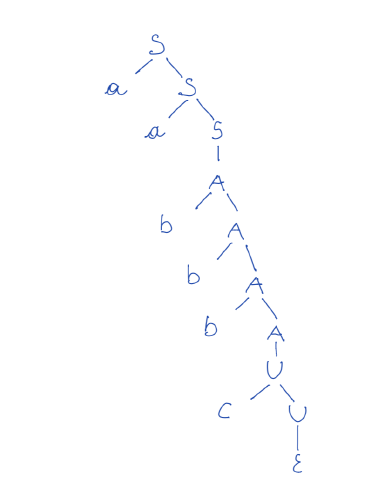
\includegraphics[width=5cm]{parse_tree_1.png}
\caption{Parse tree for the string aabbbc}
  \label{parsetree}
\end{figure}




\begin{figure}
  \centering
    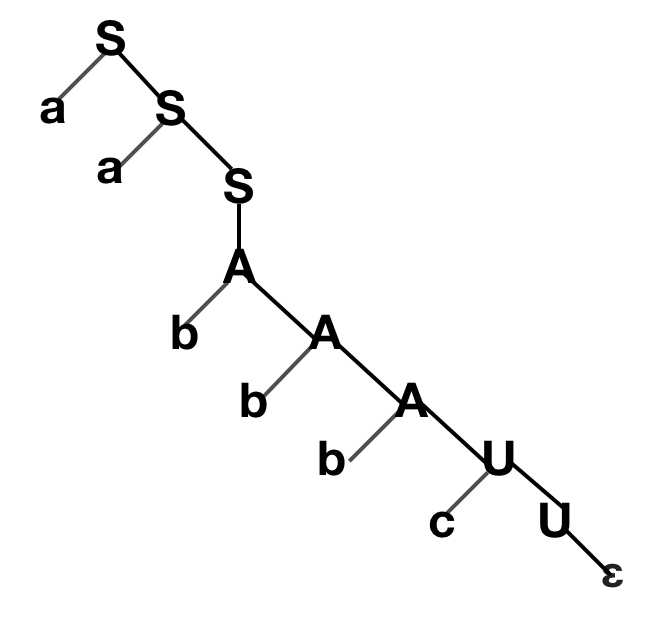
\includegraphics[width=5cm]{parse_tree_lecture2.png}
\caption{Wrong parse tree for the string aabbbc}
  \label{parsetreewrong}
\end{figure}


Regular grammars correspond to Finite State Automata (FSA). The FSA accepting the language $a^{*}b^{*}c^{*}$ 
is given in Figure \ref{fsa}.

\begin{figure}
  \centering
\begin{center}
    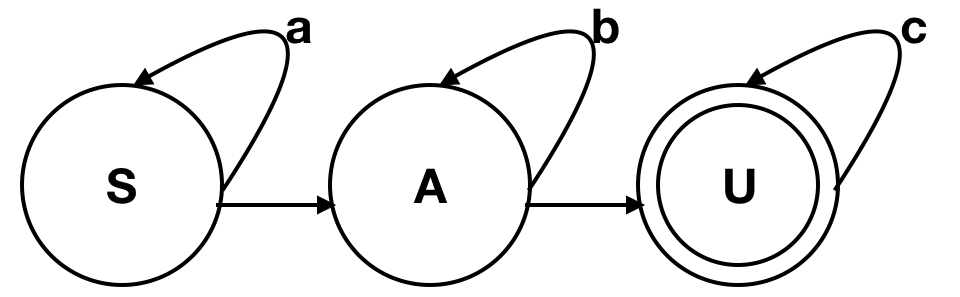
\includegraphics[width=5cm]{finite_state_automata.png}
\end{center}
\caption{FSA for the language $a^{*}b^{*}c^{*}$}
  \label{fsa}
\end{figure}

\section{Context-Free Grammar}
A contex-free grammar relaxes some restrictions of regular grammars.
In particular, the right-hand side of a production can be any string over the
alphabet $T \cup NT$:

\begin{definition}
A {\emph{context-free grammar}}  (CFG) has $l \in NT $ and $ r =  (T \cup NT)^*$.
\end{definition}


\begin{example}
The CFG grammar defining the language 
\verb|{|$a^{n}b^{n}\mid n \geq 1$\verb|}| 
is
 $$S ::= aSb \mid ab$$.
 The CFG grammar defining the language 
\verb|{|$a^{n}b^{n}\mid n \geq 0$\verb|}| 
is
 $$S ::= aSb \mid \epsilon$$.
Note that there isn't a unique way to give a grammar. One can always introduce
more non terminals as in the following grammar:
$$\begin{array}{lll}
S & ::= &  aSb \mid X \\
X & ::= &  ab 
\end{array}$$
\end{example}


Context-free grammars correspond to push down automata.


\section{Context-sensitive grammars}
Context-sensitive grammars do not impose any restrictions
on the left and right-hand side of a production. Such a grammar
is needed to recognize a language of the form
           $$a^{n}b^{n}c^{n}$$
Intuitively, one could also argue that the above language cannot be context-free since
one needs an additional memory to remember the number of $b$'s. This is not possible
in a PDA.

\section{How to solve the ambiguity of grammars}
Consider the following grammar of arithmetic expressions: 
$$ E ::= a \mid  b  \mid  c  \mid  E + E $$
The expression $a+b+c$ belong to the language of arithmetic,
as shown in Figure \ref{parsetreearith}. However, note that the expression can be parsed
in a different way. We call such a grammar {\color{red} ambiguous}.

\begin{figure}
  \centering
   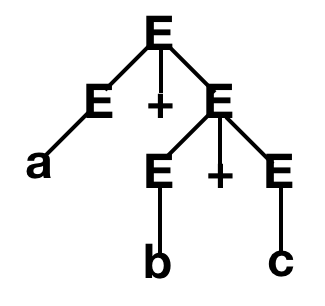
\includegraphics[width=5cm]{right_associative_parse_tree.png}
    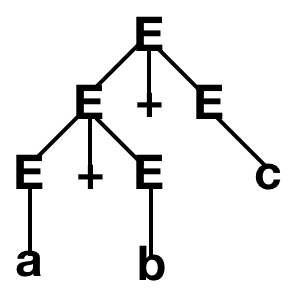
\includegraphics[width=5cm]{left_associative_parse_tree.png}
\caption{Parse trees for the string a+b+c}
  \label{parsetreearith}
\end{figure}

\begin{definition}
A grammar is ambiguous is there is exists a string in the language with more than one parse tree. 
\end{definition}

We want to avoid ambiguous grammars because the compiler will not know what code to generate.
\newline\newline
To avoid this problem the grammar can be rewritten to impose  the use of parentheses. The user would have to write
either $(a+(b+c))$ or $((a+b)+c)$.


\subsection*{Left-associativity}
Another solution is to rely on a predefined default case, which in this case would be $(a+b)+c$. In other words, 
we assume addition to be left associative. This can be directly expressed in the grammar by making use of an additional nonterminal:
$$\begin{array}{lll}
E  & ::= &  E + F \mid F \\
F & ::= & a \mid b \mid  c
\end{array}$$


\subsection*{Priority}
Let us now extend the language with multiplication:
$$ E ::= a\mid b \mid c \mid E + E \mid E * E$$
We assume that both + and * are left-associative, however, we still have one more
decision to take.  Consider the expression  
\begin{center}
a + b * c 
\end{center}
do we read it as 
\begin{center}
a + ( b * c) or (a + b) * c ? 
\end{center}
 The default case, used by a
compiler, is that multiplication has higher priority over addition, therefore
 a + ( b * c) will be the default reading.
 
\subsection*{Non Ambiguous Grammar}
We can express both association and priority in 
an non ambiguous grammar, as
defined below:
%Ideally we want to write non ambiguous grammars. For example, we can write a non ambiguous parse tree that captures left associativity. 
%\newline\newline
%E ::= $a \mid b \mid c \mid E + F \mid E * E$ \newline
%E ::= $F \mid E + F$ \newline
%F ::= $a \mid b \mid c$
%
$$\begin{array}{lll}
E & ::= & E + F \mid F \\
F & ::= & F * T \mid T\\
T & ::= & a \mid b \mid c 
\end{array}$$

%\begin{center}
%   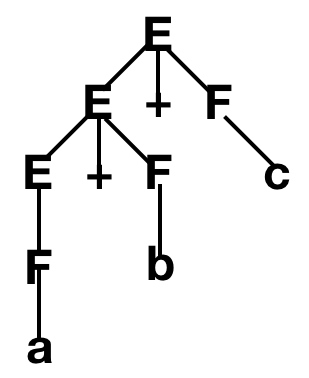
\includegraphics[width=5cm]{non_amb_tree.png}
%\end{center}

\subsection*{Abstract Syntax Trees}
After having determined that the program is syntactically correct, a compiler translates the parse tree into
a structure containing only terminal symbols, called  {\color{red} {\emph{abstract syntax tree}}}. For example, the 
abstract syntax tree representing the expression $a*b+c$ is given in Figure \ref{ast}.

\begin{figure}
  \centering
   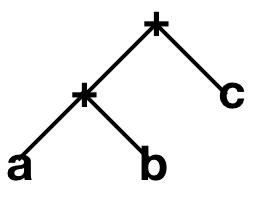
\includegraphics[width=5cm]{abs_tree.png}
\caption{Abstract syntax tree for $a*b+c$ }
  \label{ast}
\end{figure}


\subsection*{Infix, Prefix and Postfix}
So far we mainly made use of infix notation for expressions, however languages use
other notations:\\
{\color{red} Prefix} : (+ a b), (+ (+ a b) c) 
\newline
{\color{red} Postfix} : (a b +)

\subsection*{References}
 
The following have been suggested by students:

\begin{verbatim}
http://kilby.stanford.edu/~rvg/154/handouts/grammars.html
 
http://www.cs.ru.nl/~herman/onderwijs/FLGA/lecture6.pdf
 
https://www.tutorialspoint.com/automata_theory/chomsky_classification_of_grammars.htm
\end{verbatim}
\end{document}

